\documentclass[10pt,a4paper]{article}
\usepackage{iftex}
\ifPDFTeX\usepackage[utf8]{inputenc}\usepackage[T1]{fontenc}\usepackage{lmodern}
\else\usepackage{fontspec}\fi
\usepackage[margin=2cm]{geometry}\usepackage{longtable}\usepackage{array}
\usepackage{tikz}\usetikzlibrary{positioning,arrows.meta}
\usepackage{xurl}\usepackage[hidelinks]{hyperref}\usepackage{fancyvrb}
\setlength{\parskip}{4pt}\setlength{\parindent}{0pt}\setlength{\tabcolsep}{3pt}
\tikzset{>={Latex}}
\title{Literature search report -- Example project}\author{scitech-librarian 3.2}\date{\today}
\begin{document}\maketitle
Generated by scitech-librarian 3.2 (report level: simple). Every number below is reproducible from the archived research directory \texttt{lit}.

{\scriptsize\begin{longtable}{p{0.291\linewidth}p{0.664\linewidth}}
\hline
\textbf{Item} & \textbf{Value} \\ \hline
\endhead
Search dates & 2026-08-28 to 2026-08-28 \\
Project & Example project \\
Description & the four example blocks of queries.example.json, searched twice, plus a reference list from a colleague \\
Sources & 2 automated run(s), 1 manual source(s) \\
Blocks & NOV, MLP, PSC, QC \\
Backends / sources & openalex, arxiv, inspire, semanticscholar, ads, scopus, manual:reference-list \\
Mode & full fetch, up to 300 records per block and backend \\
Non-curated venue filter & on \\
Open-access lookup & not run \\
Journal metrics & on file for 599 journals \\
Filters & sources=all \\
\hline
\end{longtable}}
\section*{Sources}
Every search that feeds this report, oldest first. 'New here' counts unique records that no earlier source had found -- what each search added.

{\scriptsize\begin{longtable}{p{0.136\linewidth}p{0.071\linewidth}p{0.143\linewidth}p{0.086\linewidth}p{0.079\linewidth}p{0.086\linewidth}p{0.293\linewidth}}
\hline
\textbf{Source} & \textbf{Kind} & \textbf{Date} & \textbf{Method} & \textbf{Records} & \textbf{New here} & \textbf{Label / origin} \\ \hline
\endhead
20260828T091142 & run & 2026-08-28 09:11 & database & 5 & 5 & first pass (OpenAlex only, NOV + MLP) \\
20260828T100120 & run & 2026-08-28 10:01 & database & 2931 & 2211 & full run, six databases \\
reference-list & manual & 2026-08-28 11:30 & citation & 8 & 2 & reference list of a review article \\
\hline
\end{longtable}}
\section*{Search strategy}
Each block is one structural query -- a conjunction of synonym groups, (a OR b) AND (c OR d) -- rendered into every backend's native grammar. The strings below are exactly what was sent (PRISMA-S item 8), from the most recent run of each block.

\subsection*{Block NOV: EXAMPLE NOVELTY CHECK: origami metamaterials as topological acoustic pumps}
Purpose: novelty-check pattern -- a SMALL number is the good outcome; read every hit by hand before claiming a gap

\begin{Verbatim}[fontsize=\scriptsize]
(origami OR kirigami) AND (acoustic metamaterial OR phononic crystal) AND (topological pumping OR 
Thouless pump OR edge state)
\end{Verbatim}
{\scriptsize\begin{longtable}{p{0.219\linewidth}p{0.736\linewidth}}
\hline
\textbf{Backend} & \textbf{Query string sent} \\ \hline
\endhead
openalex & (origami OR kirigami) AND ("acoustic metamaterial" OR "phononic crystal") AND ("topological pumping" OR "Thouless pump" OR "edge state") \\
arxiv & (all:"origami" OR all:"kirigami") AND (all:"acoustic metamaterial" OR all:"phononic crystal") \\
inspire & ("origami" or "kirigami") and ("acoustic metamaterial" or "phononic crystal") and ("topological pumping" or "Thouless pump" or "edge state") \\
semanticscholar & ("origami" | "kirigami") + ("acoustic metamaterial" | "phononic crystal") + ("topological pumping" | "Thouless pump" | "edge state") \\
ads & (abs:"origami" OR abs:"kirigami") AND (abs:"acoustic metamaterial" OR abs:"phononic crystal") AND (abs:"topological pumping" OR abs:"Thouless pump" OR abs:"edge state") \\
scopus & TITLE-ABS-KEY(origami OR kirigami) AND TITLE-ABS-KEY("acoustic metamaterial" OR "phononic crystal") AND TITLE-ABS-KEY("topological pumping" OR "Thouless pump" OR "edge state") \\
\hline
\end{longtable}}
\subsection*{Block MLP: Machine-learned interatomic potentials for amorphous materials}
Purpose: a narrower intersection -- expect hundreds; good for testing record fetch and RIS export

\begin{Verbatim}[fontsize=\scriptsize]
(machine learning potential OR machine-learned interatomic potential OR neural network potential) AND 
(amorphous OR glass OR disordered solid) AND (molecular dynamics OR structure prediction)
\end{Verbatim}
arXiv receives groups {[}0, 1{]} only (nested-boolean limitation).

{\scriptsize\begin{longtable}{p{0.219\linewidth}p{0.736\linewidth}}
\hline
\textbf{Backend} & \textbf{Query string sent} \\ \hline
\endhead
openalex & ("machine learning potential" OR "machine-learned interatomic potential" OR "neural network potential") AND (amorphous OR glass OR "disordered solid") AND ("molecular dynamics" OR "structure prediction") \\
arxiv & (all:"machine learning potential" OR all:"machine-learned interatomic potential" OR all:"neural network potential") AND (all:"amorphous" OR all:"glass" OR all:"disordered solid") \\
inspire & ("machine learning potential" or "machine-learned interatomic potential" or "neural network potential") and ("amorphous" or "glass" or "disordered solid") and ("molecular dynamics" or "structure prediction") \\
semanticscholar & ("machine learning potential" | "machine-learned interatomic potential" | "neural network potential") + ("amorphous" | "glass" | "disordered solid") + ("molecular dynamics" | "structure prediction") \\
ads & (abs:"machine learning potential" OR abs:"machine-learned interatomic potential" OR abs:"neural network potential") AND (abs:"amorphous" OR abs:"glass" OR abs:"disordered solid") AND (abs:"molecular dynamics" OR abs:"structure prediction") \\
scopus & TITLE-ABS-KEY("machine learning potential" OR "machine-learned interatomic potential" OR "neural network potential") AND TITLE-ABS-KEY(amorphous OR glass OR "disordered solid") AND TITLE-ABS-KEY("molecular dynamics" OR "structure prediction") \\
\hline
\end{longtable}}
\subsection*{Block PSC: Perovskite solar cell degradation under humidity}
Purpose: grounding block -- expect thousands of hits; use it to sanity-check that every backend is reachable and the counts are plausible

\begin{Verbatim}[fontsize=\scriptsize]
(perovskite solar cell OR halide perovskite photovoltaic) AND (degradation OR stability OR encapsulation)
 AND (humidity OR moisture OR water ingress)
\end{Verbatim}
{\scriptsize\begin{longtable}{p{0.219\linewidth}p{0.736\linewidth}}
\hline
\textbf{Backend} & \textbf{Query string sent} \\ \hline
\endhead
openalex & ("perovskite solar cell" OR "halide perovskite photovoltaic") AND (degradation OR stability OR encapsulation) AND (humidity OR moisture OR "water ingress") \\
arxiv & (all:"perovskite solar cell" OR all:"halide perovskite photovoltaic") AND (all:"degradation" OR all:"stability" OR all:"encapsulation") \\
inspire & ("perovskite solar cell" or "halide perovskite photovoltaic") and ("degradation" or "stability" or "encapsulation") and ("humidity" or "moisture" or "water ingress") \\
semanticscholar & ("perovskite solar cell" | "halide perovskite photovoltaic") + ("degradation" | "stability" | "encapsulation") + ("humidity" | "moisture" | "water ingress") \\
ads & (abs:"perovskite solar cell" OR abs:"halide perovskite photovoltaic") AND (abs:"degradation" OR abs:"stability" OR abs:"encapsulation") AND (abs:"humidity" OR abs:"moisture" OR abs:"water ingress") \\
scopus & TITLE-ABS-KEY("perovskite solar cell" OR "halide perovskite photovoltaic") AND TITLE-ABS-KEY(degradation OR stability OR encapsulation) AND TITLE-ABS-KEY(humidity OR moisture OR "water ingress") \\
\hline
\end{longtable}}
\subsection*{Block QC: Quasicrystal photonics (arXiv-tuned example)}
Purpose: demonstrates arxiv\_groups: arXiv chokes on deeply nested booleans, so name the two groups it should get

\begin{Verbatim}[fontsize=\scriptsize]
(quasicrystal OR quasiperiodic lattice) AND (photonic OR waveguide OR optical lattice) AND (localization 
OR critical states OR fractal spectrum)
\end{Verbatim}
arXiv receives groups {[}0, 2{]} only (nested-boolean limitation).

{\scriptsize\begin{longtable}{p{0.219\linewidth}p{0.736\linewidth}}
\hline
\textbf{Backend} & \textbf{Query string sent} \\ \hline
\endhead
openalex & (quasicrystal OR "quasiperiodic lattice") AND (photonic OR waveguide OR "optical lattice") AND (localization OR "critical states" OR "fractal spectrum") \\
arxiv & (all:"quasicrystal" OR all:"quasiperiodic lattice") AND (all:"localization" OR all:"critical states" OR all:"fractal spectrum") \\
inspire & ("quasicrystal" or "quasiperiodic lattice") and ("photonic" or "waveguide" or "optical lattice") and ("localization" or "critical states" or "fractal spectrum") \\
semanticscholar & ("quasicrystal" | "quasiperiodic lattice") + ("photonic" | "waveguide" | "optical lattice") + ("localization" | "critical states" | "fractal spectrum") \\
ads & (abs:"quasicrystal" OR abs:"quasiperiodic lattice") AND (abs:"photonic" OR abs:"waveguide" OR abs:"optical lattice") AND (abs:"localization" OR abs:"critical states" OR abs:"fractal spectrum") \\
scopus & TITLE-ABS-KEY(quasicrystal OR "quasiperiodic lattice") AND TITLE-ABS-KEY(photonic OR waveguide OR "optical lattice") AND TITLE-ABS-KEY(localization OR "critical states" OR "fractal spectrum") \\
\hline
\end{longtable}}
\section*{Results summary}
{\scriptsize\begin{longtable}{p{0.054\linewidth}p{0.072\linewidth}p{0.054\linewidth}p{0.066\linewidth}p{0.114\linewidth}p{0.054\linewidth}p{0.060\linewidth}p{0.149\linewidth}p{0.084\linewidth}p{0.078\linewidth}p{0.060\linewidth}}
\hline
\textbf{Block} & \textbf{openalex} & \textbf{arxiv} & \textbf{inspire} & \textbf{semanticscholar} & \textbf{ads} & \textbf{scopus} & \textbf{manual:reference-list} & \textbf{Identified} & \textbf{Retrieved} & \textbf{Unique} \\ \hline
\endhead
NOV & 0 & 0 & 0 & 0 & 0 & 0 & - & 0 & 0 & 0 \\
MLP & 478 & 138 & 0 & 109 & 203 & 149 & 8 & 1,085 & 815 & 446 \\
PSC & 4567 & 175 & 0 & 2968 & 2179 & 4731 & - & 14,620 & 1275 & 1163 \\
QC & 154 & 414 & 17 & 122 & 206 & 65 & - & 978 & 854 & 609 \\
Total & 5,199 & 727 & 17 & 3,199 & 2,588 & 4,945 & 8 & 16,683 & 2944 & 2218 \\
\hline
\end{longtable}}
Identified = database hit counts (not comparable across backends: proximity operators are dropped and stemming differs); summed over runs, and for manual sources the number of records ingested. Retrieved = records actually downloaded after the venue filter, capped by \texttt{--limit}. Unique = after DOI/title deduplication across all sources.

\section*{Timeline}
Per-block hit totals in each automated run (sum over backends), oldest first; drift shows how the indexes -- or the queries -- changed.

{\scriptsize\begin{longtable}{p{0.180\linewidth}p{0.381\linewidth}p{0.381\linewidth}}
\hline
\textbf{Block} & \textbf{20260828T091142} & \textbf{20260828T100120} \\ \hline
\endhead
NOV & 0 & 0 \\
MLP & 239 & 838 \\
PSC & - & 14,620 \\
QC & - & 978 \\
\hline
\end{longtable}}
\subsection*{When records entered the project}
{\scriptsize\begin{longtable}{p{0.318\linewidth}p{0.637\linewidth}}
\hline
\textbf{Month} & \textbf{Records first seen} \\ \hline
\endhead
2026-08 & 2218 \\
\hline
\end{longtable}}
\section*{PRISMA 2020 flow}
\begin{center}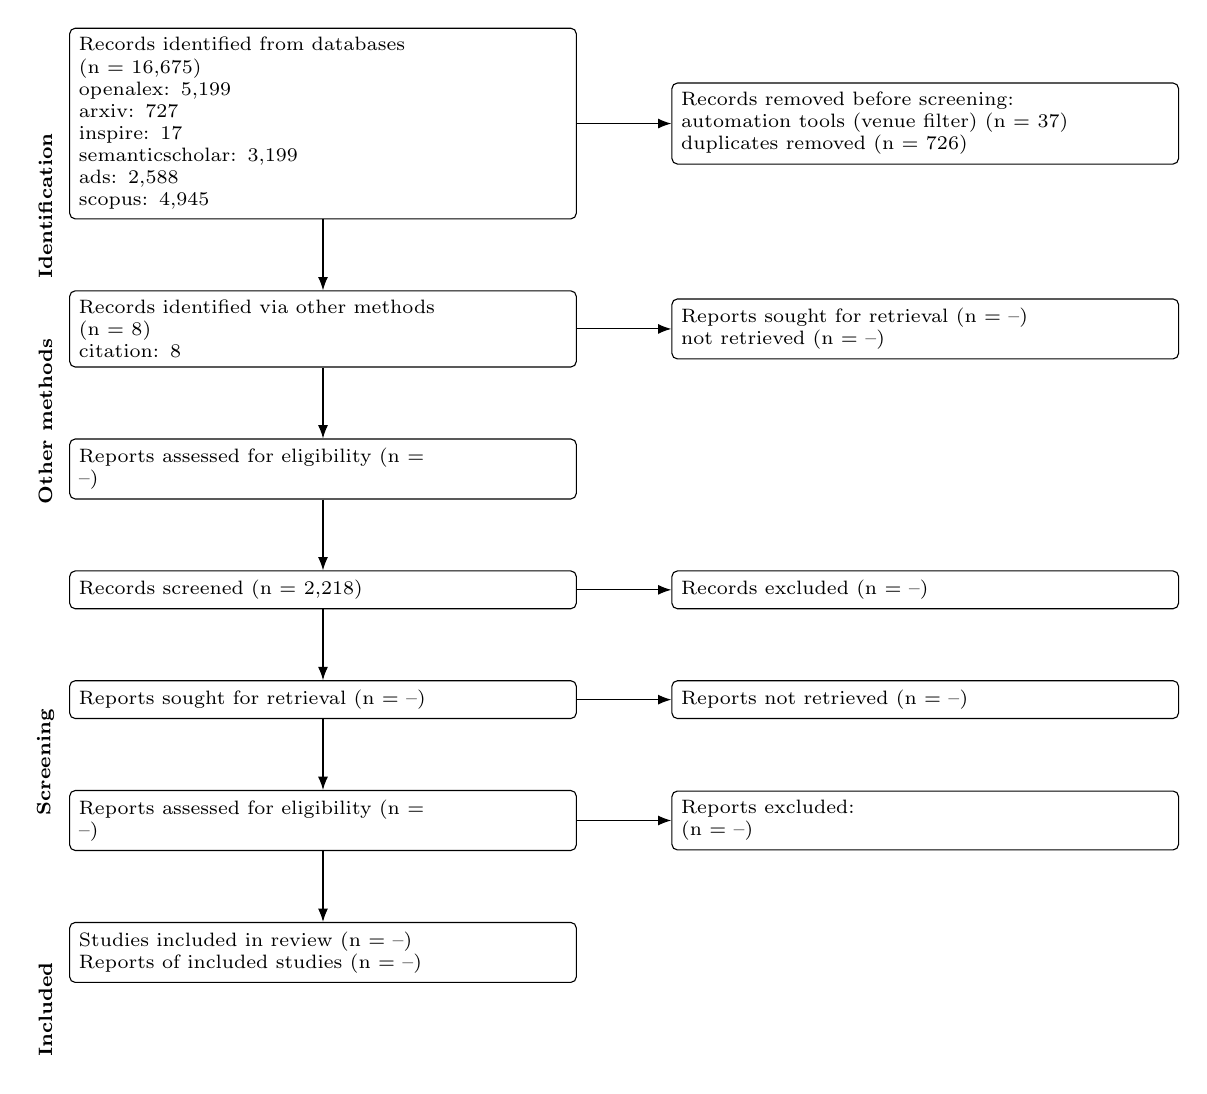
\begin{tikzpicture}[node distance=9mm and 12mm,
  box/.style={draw, rounded corners=2pt, text width=62mm, align=left, font=\scriptsize},
  lab/.style={rotate=90, font=\scriptsize\bfseries}]
\node[box] (id) {Records identified from databases \\ (n = 16,675) \\ openalex: 5,199 \\ arxiv: 727 \\ inspire: 17 \\ semanticscholar: 3,199 \\ ads: 2,588 \\ scopus: 4,945};
\node[box, right=of id] (idr) {Records removed before screening: \\ automation tools (venue filter) (n = 37) \\ duplicates removed (n = 726)};
\node[box, below=of id] (ot) {Records identified via other methods \\ (n = 8) \\ citation: 8};
\node[box, right=of ot] (otr) {Reports sought for retrieval (n = --) \\ not retrieved (n = --)};
\node[box, below=of ot] (ota) {Reports assessed for eligibility (n = \\ --)};
\node[lab, left=3mm of ot] {Other methods};
\draw[->] (ot) -- (otr); \draw[->] (ot) -- (ota); \draw[->] (id) -- (ot);
\node[box, below=of ota] (sc) {Records screened (n = 2,218)};
\node[box, right=of sc] (scr) {Records excluded (n = --)};
\node[box, below=of sc] (sc2) {Reports sought for retrieval (n = --)};
\node[box, right=of sc2] (sc2r) {Reports not retrieved (n = --)};
\node[box, below=of sc2] (sc3) {Reports assessed for eligibility (n = \\ --)};
\node[box, right=of sc3] (sc3r) {Reports excluded: \\ (n = --)};
\node[box, below=of sc3] (inc) {Studies included in review (n = --) \\ Reports of included studies (n = --)};
\node[lab, left=3mm of id] {Identification};
\node[lab, left=3mm of sc2] {Screening};
\node[lab, left=3mm of inc] {Included};
\draw[->] (id) -- (idr); \draw[->] (sc) -- (scr); \draw[->] (sc2) -- (sc2r);
\draw[->] (sc3) -- (sc3r);
\draw[->] (ota) -- (sc); \draw[->] (sc) -- (sc2); \draw[->] (sc2) -- (sc3);
\draw[->] (sc3) -- (inc);
\end{tikzpicture}\end{center}
{\scriptsize\begin{longtable}{p{0.655\linewidth}p{0.300\linewidth}}
\hline
\textbf{Stage} & \textbf{n} \\ \hline
\endhead
Records identified from databases & 16,675 \\
  openalex & 5,199 \\
  arxiv & 727 \\
  inspire & 17 \\
  semanticscholar & 3,199 \\
  ads & 2,588 \\
  scopus & 4,945 \\
Records identified via other methods & 8 \\
  citation & 8 \\
Records retrieved (downloaded / ingested) & 2,981 \\
Removed before screening: automation (non-curated venues) & 37 \\
Removed before screening: duplicates & 726 \\
Records to screen (unique) & 2,218 \\
Records screened & 2,218 (assumed = unique) \\
Records excluded at screening & -- \\
Reports sought for retrieval & -- \\
Reports not retrieved & -- \\
Reports assessed for eligibility & -- \\
Other methods: reports sought & -- \\
Other methods: reports not retrieved & -- \\
Other methods: reports assessed & -- \\
Studies included & -- \\
Reports of included studies & -- \\
\hline
\end{longtable}}
Automation stages are computed from the data; '--' marks manual stages not yet recorded in screening.json. Note that 'identified' counts hits reported by each database while 'retrieved' is what was downloaded within \texttt{--limit}, so the two differ on large blocks.

\subsection*{PRISMA-S search-reporting checklist}
{\scriptsize\begin{longtable}{p{0.072\linewidth}p{0.296\linewidth}p{0.574\linewidth}}
\hline
\textbf{Item} & \textbf{Requirement} & \textbf{This search} \\ \hline
\endhead
1 & Database name & openalex, arxiv, inspire, semanticscholar, ads, scopus (documented public APIs) \\
2 & Multi-database searching & 6 databases, one structural query per block rendered into each native grammar; see Search strategy \\
3 & Study registries & not applicable \\
4 & Online resources and browsing & none recorded \\
5 & Citation searching & reference-list \\
6 & Contacts & none recorded \\
7 & Other methods & none \\
8 & Full search strategies & reported verbatim per backend under Search strategy; archived in queries.json of each run \\
9 & Limits and restrictions & record download capped at 300 per block and backend, most-cited first; no date, language or document-type limits applied; report filters: sources=all \\
10 & Search filters & venue filter on: records from non-curated repositories (Zenodo, Figshare, SSRN...) removed \\
11 & Prior work & none \\
12 & Updates & 2 run(s) combined; see Timeline \\
13 & Dates of searches & searched on 2026-08-28 to 2026-08-28 \\
14 & Peer review & none \\
15 & Total records & 16,675 identified from databases, 8 via other methods; 2,981 retrieved; 2,218 unique \\
16 & Deduplication & exact DOI match, else first 90 characters of the lower-cased title; 726 duplicates removed \\
\hline
\end{longtable}}
\section*{Top 10 records per block}
Deduplicated across sources, sorted by cited. The complete set is in all\_records.csv / .ris of each run.

\subsection*{Block MLP (446 unique)}
{\scriptsize\begin{longtable}{p{0.210\linewidth}p{0.210\linewidth}p{0.043\linewidth}p{0.210\linewidth}p{0.043\linewidth}p{0.111\linewidth}p{0.065\linewidth}}
\hline
\textbf{Title} & \textbf{Authors} & \textbf{Year} & \textbf{Venue} & \textbf{Cited} & \textbf{DOI} & \textbf{Scopus CiteScore} \\ \hline
\endhead
Atom-centered symmetry functions for constructing high-dimensional neural network potentials & Jörg Behler & 2011 & The Journal of Chemical Physics & 1643 & \href{https://doi.org/10.1063/1.3553717}{10.1063/1.3553717} & 5.3 (2025) \\
Realistic Atomistic Structure of Amorphous Silicon from Machine-Learning-Driven Molecular Dynamics & Volker L. Deringer; Noam Bernstein; Albert P. Bartók et al. & 2018 & The Journal of Physical Chemistry Letters & 269 & \href{https://doi.org/10.1021/acs.jpclett.8b00902}{10.1021/acs.jpclett.8b00902} & 7.8 (2025) \\
Machine-learned interatomic potentials by active learning: amorphous and liquid hafnium dioxide & Ganesh Sivaraman; Anand Narayanan Krishnamoorthy; Matthias Baur et al. & 2020 & npj Computational Materials & 195 & \href{https://doi.org/10.1038/s41524-020-00367-7}{10.1038/s41524-020-00367-7} & 17.4 (2025) \\
Machine-learned interatomic potentials by active learning: amorphous and liquid hafnium dioxide & Ganesh Sivaraman; Anand Narayanan Krishnamoorthy; Matthias Baur et al. & 2019 & Cambridge University Engineering Department Publications Database & 184 & \href{https://doi.org/10.17863/cam.55408}{10.17863/cam.55408} &  \\
Growth Mechanism and Origin of High s p<SUP>3</SUP> Content in Tetrahedral Amorphous Carbon & Caro, Miguel A.; Deringer, Volker L.; Koskinen, Jari et al. & 2018 & Phys. Rev. Lett. 120, 166101 (2018) & 178 & \href{https://doi.org/10.1103/PhysRevLett.120.166101}{10.1103/PhysRevLett.120.166101} &  \\
Constructing first-principles phase diagrams of amorphous Li<SUB>x</SUB>Si using machine-learning-assisted sampling with an evolutionary algorithm & Artrith, Nongnuch; Urban, Alexander; Ceder, Gerbrand & 2018 & The Journal of Chemical Physics 148 (24), 241711 2018 & 155 & \href{https://doi.org/10.1063/1.5017661}{10.1063/1.5017661} &  \\
Study of Li atom diffusion in amorphous Li3PO4 with neural network potential & Wenwen Li; Yasunobu Ando; Emi Minamitani et al. & 2017 & The Journal of Chemical Physics & 154 & \href{https://doi.org/10.1063/1.4997242}{10.1063/1.4997242} & 5.3 (2025) \\
Impact of the Local Environment on Li Ion Transport in Inorganic Components of Solid Electrolyte Interphases & Taiping Hu; Jianxin Tian; Fuzhi Dai et al. & 2022 & Journal of the American Chemical Society & 107 & \href{https://doi.org/10.1021/jacs.2c11521}{10.1021/jacs.2c11521} & 22 (2025) \\
Thermal conductivity modeling using machine learning potentials: application to crystalline and amorphous silicon & Qian, X.; Peng, S.; Li, X. et al. & 2019 & Materials Today Physics & 103 & \href{https://doi.org/10.1016/j.mtphys.2019.100140}{10.1016/j.mtphys.2019.100140} & 16.7 (2025) \\
A unified deep neural network potential capable of predicting thermal conductivity of silicon in different phases & Li, R.; Lee, E.; Luo, T. & 2020 & Materials Today Physics & 102 & \href{https://doi.org/10.1016/j.mtphys.2020.100181}{10.1016/j.mtphys.2020.100181} & 16.7 (2025) \\
\hline
\end{longtable}}
\subsection*{Block PSC (1163 unique)}
{\scriptsize\begin{longtable}{p{0.232\linewidth}p{0.232\linewidth}p{0.044\linewidth}p{0.156\linewidth}p{0.044\linewidth}p{0.112\linewidth}p{0.073\linewidth}}
\hline
\textbf{Title} & \textbf{Authors} & \textbf{Year} & \textbf{Venue} & \textbf{Cited} & \textbf{DOI} & \textbf{Scopus CiteScore} \\ \hline
\endhead
Incorporation of rubidium cations into perovskite solar cells improves photovoltaic performance & Michael Saliba; Taisuke Matsui; Konrad Domanski et al. & 2016 & Science & 3691 & \href{https://doi.org/10.1126/science.aah5557}{10.1126/science.aah5557} &  \\
High-efficiency two-dimensional Ruddlesden–Popper perovskite solar cells & Hsinhan Tsai; Wanyi Nie; Jean‐Christophe Blancon et al. & 2016 & Nature & 3360 & \href{https://doi.org/10.1038/nature18306}{10.1038/nature18306} &  \\
Efficient, stable and scalable perovskite solar cells using poly(3-hexylthiophene) & Jung, Eui Hyuk; Jeon, Nam Joong; Park, Eun Young et al. & 2019 & Nature & 2318 & \href{https://doi.org/10.1038/s41586-019-1036-3}{10.1038/s41586-019-1036-3} &  \\
A Layered Hybrid Perovskite Solar‐Cell Absorber with Enhanced Moisture Stability & Ian C. P. Smith; Eric T. Hoke; Diego Solís-Ibarra et al. & 2014 & Angewandte Chemie International Edition & 2006 & \href{https://doi.org/10.1002/anie.201406466}{10.1002/anie.201406466} & 25.7 (2025) \\
Review of recent progress in chemical stability of perovskite solar cells & Guangda Niu; Xudong Guo; Liduo Wang & 2014 & Journal of Materials Chemistry A & 1942 & \href{https://doi.org/10.1039/c4ta04994b}{10.1039/c4ta04994b} & 14.5 (2025) \\
Understanding Degradation Mechanisms and Improving Stability of Perovskite Photovoltaics & Caleb C. Boyd; Rongrong Cheacharoen; Tomas Leijtens et al. & 2018 & Chemical Reviews & 1767 & \href{https://doi.org/10.1021/acs.chemrev.8b00336}{10.1021/acs.chemrev.8b00336} & 109.1 (2025) \\
Formamidinium and Cesium Hybridization for Photo- and Moisture-Stable Perovskite Solar Cell & Lee, Jin-Wook; Kim, Deok-Hwan; Kim, Hui-Seon et al. & 2015 & Advanced Energy Materials & 1661 & \href{https://doi.org/10.1002/aenm.201501310}{10.1002/aenm.201501310} & 39.9 (2025) \\
23.6\%-efficient monolithic perovskite/silicon tandem solar cells with improved stability & Kevin A. Bush; Axel F. Palmstrom; Zhengshan J. Yu et al. & 2017 & Nature Energy & 1533 & \href{https://doi.org/10.1038/nenergy.2017.9}{10.1038/nenergy.2017.9} & 78.4 (2025) \\
Investigation of CH 3 NH 3 PbI 3 Degradation Rates and Mechanisms in Controlled Humidity Environments Using in Situ Techniques & Jinli Yang; Braden D. Siempelkamp; Dianyi Liu et al. & 2015 & ACS Nano & 1342 & \href{https://doi.org/10.1021/nn506864k}{10.1021/nn506864k} & 23.1 (2025) \\
Carbon Nanotube/Polymer Composites as a Highly Stable Hole Collection Layer in Perovskite Solar Cells & Severin N. Habisreutinger; Tomas Leijtens; Giles E. Eperon et al. & 2014 & Nano Letters & 1198 & \href{https://doi.org/10.1021/nl501982b}{10.1021/nl501982b} & 13.5 (2025) \\
\hline
\end{longtable}}
\subsection*{Block QC (609 unique)}
{\scriptsize\begin{longtable}{p{0.246\linewidth}p{0.246\linewidth}p{0.044\linewidth}p{0.104\linewidth}p{0.044\linewidth}p{0.131\linewidth}p{0.077\linewidth}}
\hline
\textbf{Title} & \textbf{Authors} & \textbf{Year} & \textbf{Venue} & \textbf{Cited} & \textbf{DOI} & \textbf{Scopus CiteScore} \\ \hline
\endhead
Transport and Anderson localization in disordered two-dimensional photonic lattices & Schwartz, Tal; Bartal, Guy; Fishman, Shmuel et al. & 2007 &  & 1329 & \href{https://doi.org/10.1038/nature05623}{10.1038/nature05623} &  \\
Observation of two-dimensional discrete solitons in optically induced nonlinear photonic lattices & Fleischer, Jason W.; Segev, Mordechai; Efremidis, Nikolaos K. et al. & 2003 &  & 1039 & \href{https://doi.org/10.1038/nature01452}{10.1038/nature01452} &  \\
Hyperuniform states of matter & Salvatore Torquato & 2018 & Physics Reports & 501 & \href{https://doi.org/10.1016/j.physrep.2018.03.001}{10.1016/j.physrep.2018.03.001} & 54.4 (2025) \\
Localization and delocalization of light in photonic moiré lattices & Wang, Peng; Zheng, Yuanlin; Chen, Xianfeng et al. & 2020 & Nature 577, 42-46(2020) & 482 & \href{https://doi.org/10.1038/s41586-019-1851-6}{10.1038/s41586-019-1851-6} &  \\
Decoherence and Disorder in Quantum Walks: From Ballistic Spread to Localization & Schreiber, A.; Cassemiro, K. N.; Potoček, V. et al. & 2011 &  & 355 & \href{https://doi.org/10.1103/PhysRevLett.106.180403}{10.1103/PhysRevLett.106.180403} &  \\
Delocalization of a disordered bosonic system by repulsive interactions & B. Deissler; Matteo Zaccanti; G. Roati et al. & 2010 & Nature Physics & 273 & \href{https://doi.org/10.1038/nphys1635}{10.1038/nphys1635} & 29.4 (2025) \\
Topological triple phase transition in non-Hermitian Floquet quasicrystals & Weidemann, Sebastian; Kremer, Mark; Longhi, Stefano et al. & 2022 & Nature & 223 & \href{https://doi.org/10.1038/s41586-021-04253-0}{10.1038/s41586-021-04253-0} &  \\
Observation of topological valley modes in an elastic hexagonal lattice & Vila, Javier; Pal, Raj Kumar; Ruzzene, Massimo & 2017 &  & 219 & \href{https://doi.org/10.1103/PhysRevB.96.134307}{10.1103/PhysRevB.96.134307} &  \\
Disorder-Enhanced Transport in Photonic Quasicrystals & Liad Levi; Mikael C. Rechtsman; Barak Freedman et al. & 2011 & Science & 205 & \href{https://doi.org/10.1126/science.1202977}{10.1126/science.1202977} &  \\
Compact localized states and flat-band generators in one dimension & Maimaiti, Wulayimu; Andreanov, Alexei; Park, Hee Chul et al. & 2017 &  & 184 & \href{https://doi.org/10.1103/PhysRevB.95.115135}{10.1103/PhysRevB.95.115135} &  \\
\hline
\end{longtable}}
\section*{Suggestions}
\begin{itemize}\item Block NOV: zero hits on every backend. Either the intersection is genuinely empty (a finding -- check the synonyms first) or one group is too narrow; try dropping one group and rerunning.\item Block PSC: openalex 4,567, semanticscholar 2,968, ads 2,179, scopus 4,731 hits -- a generic term is probably driving this; tighten a group or add a more specific one before reading.\item Block PSC: counts differ >20x across backends (175 to 4,731); grammar and coverage diverge, so do not compare these numbers -- discover here, quote one source.\item Block QC: counts differ >20x across backends (17 to 414); grammar and coverage diverge, so do not compare these numbers -- discover here, quote one source.\item Open-access status was not looked up; rerun with \texttt{--pdfs} (optionally \texttt{--pdf-blocks}) to collect legal OA PDF links via Unpaywall.\item The PRISMA flow's manual stages are empty: fill in screening.json (screened / excluded / assessed / included) and rerun report.py to complete the diagram.\end{itemize}
\end{document}